\documentclass[12pt]{article}
\usepackage{amsmath}
\usepackage{amsfonts}
\usepackage[a4paper, margin=2.5cm]{geometry}
\usepackage{graphicx}
\usepackage{setspace}
\usepackage{parskip}
\usepackage{hyperref}
\usepackage{float}
\usepackage{booktabs}
\usepackage{glossaries}
\usepackage{subcaption} % in your preamble
\onehalfspacing
\usepackage[margin=2.5cm]{geometry}
\renewcommand{\baselinestretch}{1.5}
\usepackage{fontspec}
\setmainfont{Arial}



\begin{document}











% Image optimization settings
% Configure image compression for XeTeX
\setkeys{Gin}{draft=false}

\setstretch{1.2}

\title{\Huge Autonomous Bitcoin Trading\\\vspace{1cm}\Large Documentation}
\author{
    \Large Gymnasium Thun\\
     26gs\\
    \vspace{1cm}
    \Large Submitted by:\\
    \vspace{0.5cm}
    \textbf{Juri Stoffers}\\
    \vspace{2cm}
    \Large Supervised by:\\
    \vspace{0.5cm}
    \textbf{Dr. Geoffrey Ostrin}
}

% Title page
\pagenumbering{gobble}
\maketitle
\clearpage

% Abstract
\pagenumbering{roman}
\begin{abstract}
    This thesis examines the development of an autonomous Bitcoin trading algorithm, based on the observation that human emotion leads traders to act irrationally in the markets.
    The research combines technical analysis with algorithmic trading, employing a quantitative methodology that includes data collection, strategy development using Python, and testing strategies on historical price data. The implementation involves creating a custom backtesting framework, developing rule-based trading strategies, and deploying a live trading system on a Linux based server.

\end{abstract}
\clearpage

% Continue roman numbering from abstract
\section*{Foreword}
My interest in Bitcoin began in early 2022 after reading \textit{The Bitcoin Standard by Saifedean Ammous}. The book explores the history of money and argues that Bitcoin is a revolutionary form of hard money \footnote{A form of money that maintains its value over time, offering stability and reliability} superior to traditional currencies. The book sparked an interest in me, and I was drawn into the world of crypto. As a result, I spent more and more time watching charts and losing my mind over them. The idea of making profit from these seemingly random price movements fascinated me.
Trading profitably is straightforward: sell high and buy low. The practical implementation, however, is filled with uncertainty and  fight against your own instincts and emotions.
In addition to getting into crypto I also tried to learn to code since I wanted to make money on the side without having to leave my house. The first time I learned about automated trading algorithms I thought it was one of the hardest things to do. The combination of knowledge made me admire people who code in the finance space. It felt impossible but the more I tried the closer I got to something into the direction of a trading algorithm. With my matura thesis approaching I was pretty confident that I would be able to build an automated Bitcoin trading algorithm. 






I had no idea what I was getting myself into, and if I had known before, I would probably have never started. I spent more time than I intended and completely lost myself during the summer vacation. I totally forgot about the writing part and spent a lot of time just coding. This project grew much bigger than I initially thought, but I'm proud to present both the work outcome and the learnings I gained from it.





\clearpage

% Table of contents
\pagenumbering{roman}
\tableofcontents
\clearpage

% Start main content with arabic numbering
\pagenumbering{arabic}
\setcounter{page}{1}
\section{Introduction}
This thesis explores whether I can develop an autonomous trading algorithm that can generate me a consistent profit. To that end my thesis will cover the entire development cycle of an algorithmic trading strategy. The process will include research, finding a trading strategy, backtesting, and live trading algorithm results.



The work is divided in three parts: Finding a strategy, Backtesting, and Live trading.

Finding a strategy can be done in multiple ways just by watching markets over longer time periods to get ideas, reading books about how other people were able to develope strategies and steal logic from them. In my case I will try to find a strategy by analysing the orderbook delta and identifying trends on the not stationary bitcoin price. \footnote{Not stationary means not being still or fixed in one place; moving or changing rather than remaining constant.}

Backtesting is the process of testing a trading strategy on historical data to evaluate its performance. It is used to see if the strategy is worth automating.

Live trading is the process of executing a trading strategy on a live market. Here I will see if my strategy works in the real market and how it will behave. The strategy will be automated in python. A major difference is that I will use two different python programs for the backtesting process and the live trading algorithm.  


The project requires know how in three key areas: Statistics, Programming and understanding how the cryptocurrencies market operates. I need to apply stasticial rules to check if my idea is worthless or has potential to make me a profit if I automate the execution process. Programming is just needed to make the process of testing or applyinng my ideas easy on large datasets since I have to test on timeseries up including up to 200'000 values. The algorithm will be written in Python and will run 24 hours a day seven days a week.





By the end of the project, I aim to deliver the following components:

\begin{itemize}
    \item Backtest results
    \item Trading strategy
    \item Trading algorithm programm
    \item Live execution results
\end{itemize}




\newpage

\section{Theoretical Background}








\subsection*{What is trading?}
Trading means buying and selling financial assets like stocks, cryptocurrencies, or commodities, usually with the goal of making a profit. Traders try to buy at a low price and sell at a higher one, or profit from falling prices by selling high and buying back lower. Prices in financial markets change constantly, which creates opportunities — but also risks. There are many different types of trading, depending on the chosen timeframe, strategy, and how trades are managed. Losing is part of every strategy the goal is to lose less money than you win.
As trading is often seen as an easy way to make money it is important to understand that it is not easy. It is a skill that requires a lot of time and effort to master. Type of trading strategy does not matter there is no easy or fast way to success in trading. 

\subsubsection*{Algorithmic Trading}
In this thesis I will try to find success in the algorithmic trading niche, also know as Algo-trading or automated trading. This is a type of trading which uses computer programs to execute trades in finacial markets based on predefined rules or mathematical models.  Inside of algorithmic trading there are again many different types. Some examples are: statistical arbitrage, trend following, and High-Frequency Trading. In terms of logic all these are not related at all and strategies are often very complex in these areas. 

My strategy is best descirbed as a statistical signal-based strategy. As I try to find a metric that shows statistical evidence on which I can capitalized on. In financial markets we can profit by betting on a volatilty change \footnote{a measure of how much and how quickly the price of a trading instrument fluctuates over time} or directional bias. Capitalizing from directional bias is as simple as buying if your directional bias positive and selling if we have a negative directional bias. (I am reffering to positive and negative returns)















\newpage
\subsection*{Efficient markets}
Making consistent profits in financial markets is difficult. Prices move in ways that often seem unpredictable, and most traders both discretionary and systematic struggle to gain a lasting edge. \footnote[1]{An edge is a consistent advantage over the market. It can be achieved through superior information, better analysis, or a unique trading approach.}One explination for this is the Efficient market hypothesis (EMH) which suggest that asset prices already reflect all available information, leaving little room for profitable oppertunities.






If the EMH were fully accurate in practice, then even the most advanced trading algorithms and best discretionary traders would not be able to consistently beat the market. \footnote[2]{Beating the market means achieving a higher ROI ("Return on Investment") than a certain benchmark. A common benchmark is the S\&P 500, which is an index including the 500 largest companies listed on U.S. stock exchanges. The S\&P 500 has had an average yearly return of about 10.33\% since 1957} Yet markets are not perfectly efficient, being heavily influenced by emotion, fear, and herd behaviour. Traders often fail to act on clear signals simply because it is psychologically hard to buy on a red day or sell while everybody is full of euphoria.


To make things even better depending on where you trade market can change in efficient. But still some of the most valuable assets like stocks, gold and Bitcoin prices are a reflection of human emotion pricing in information. Especially now with Trump in office a lot of volatility came in with big opportunities

Depending on the timeframe there are still a lot inefficiencies from which individuals can make a profit from. I will try to act on short term inefficiencies with my trading algorithm because I only have about one month for the live test and it would not make sense to run an algorithm which holds a trade over weeks and takes a trade every two months. In addition my initial idea when I started of with my matura thesis was already based on short term signals.§

It is possible to make a profit in the markets but it is not easy, not for everyone, and needs dedication. I am pretty sure I am able to make a profit. The question rather is if it is possible to do so in the limited time I have and at what scale.


\newpage








\subsection*{Development of a Systematic Strategy}


A systematic strategy is a trading strategy which uses fixed entry and exit conditions. Entry conditions in systematic trading strategies can vary from entries based on news, technical indicators, or other external factors. In contrast to discretionary trading where the trader decides whether to enter or exit a trade based on human emotion or intuition.

\textbf{Idea Generation:}
The systematic strategy has to be based on a hypothesis that once signal X occurs the market is wrong and we can profit from the market correcting back to a fair value. Finding an idea to test on if there is an edge to it is the first step. This can be done by copying other strategies and applying them in a different way or in a different market. The approach I took was trying to make a discretionary strategy into a systematic one.



\textbf{Backtesting:}
After coming up with an idea we have to make a stric entry and exit conditions. We test the rules on historical data. This allows the developer to evaluate how the strategy would have performed in the past. This allows us to get a hint on how the strategy would perform in the future and if it is worth automating. 

\textbf{Optimization and Robustness Testing:}
After initial tests, parameters can be adjusted. A simple example would be adjusting the holding time of a trade. If a strategy ends up to not be profitable with a trade holding time of 15 minutes this doesn't mean the strategy is not profitable. It just means that the strategy is not profitable with a trade holding time of 15 minutes. Some inefficiencies can be corrected in minutes others might take a day or two. Holding time is a simple example which doesn't bring a lot of risk with it if we test on different holding times. As long as we use a limited amount and have clear differences between the different holding times we can be sure that the strategy is robust. The biggest risk we face with backtesting is that we might overfit the strategy to the past data. An overfitted strategy looks great on historical data but will fail in the live market.

\textbf{Live Execution:}
If the backtesting results are promising and the strategy appears robust, it can be deployed live. Execution is handled by a bot or script running on a server, which listens to market data and acts as soon as the conditions are met. New things have to be taken in consideration here whicha are not a problem in backtests. One such thing is the time it takes to calculate the entry and exit conditions. This is a problem, as the price might change between when the actual entry conditions occur and when the entry signal is calculated.

Throughout this process, the focus remains on consistency and measurable results. Unlike human decision-making, a systematic strategy must behave identically entry and exit conditions. This makes it possible to evaluate, improve and automate trading in a transparent way.

\newpage

\subsection*{Why trade Bitcoin?}
To prevent any misunderstanding, I want to clarify that I chose Bitcoin as an underlying asset for my trading strategy out of practicality and how my personal opinion about the asset is irrelevant. I read a few books explaining the reason for the creation of Bitcoin and the fundamentals behind it. I personally believe in the narrative of Bitcoin as a decentralized and inflation-secure asset. However, this belief of mine plays no role in my trading algorithm. The goal of the trading algorithm is to react to signals which indicate market inefficiencies. These market inefficiencies can occur on any kind of asset in different magnitudes.
\subsubsection*{Data accessibility}
In the crypto market, real time and historical data is mostly free and accessible freely through public APIs. An API is a tool that allows programs to request and receive specific data from external services in this case, used to fetch real-time Bitcoin price and orderbook data from the coinbase crypto exchange. The data I based my strategy on is totaly free I just had to create my own timeseries in the traditional market I would have paid thousands of dollars for the data.

\subsubsection*{Modern API infrastructure}
Some crypto exchanges offer modern API infastrucutre which allow direct automate in trading. The exchange I chose Hyperliquid offers world class python implementation of their API. This allows me to carry out trades with a simple self written python script that implements their python sdk. \footnote{A python sdk is a software development kit for python. It is a collection of tools and libraries that allow developers to interact with a specific API.}

\subsubsection*{Entry barriers}
You can start trading crypto with as little as 10 USD no matter if the exchanges offers automated trading or just manual executed trades. While in the traditional market you need atleast 10'000 USD to open an account for on a broker which offers automated strategy access.



\subsubsection*{Underlying asset}
The economical fundenmentals of the asset do not matter as long as the price of the asset is determined by supply and demand inside of an orderbook.






\newpage
\section{Methodology}

\subsection*{Project Overview}
The aim of this project was to design, test, and deploy a fully automated trading strategy for Bitcoin. My development process consisted of four main stages. First, historical price data was collected through a public exchange API \footnote[1]{API stands for Application Programming Interface. It is a tool that allows programs to request and receive specific data from external services in this case, used to fetch real-time Bitcoin price and orderbook data from the coinbase crypto exchange.} and fetched in one-minute intervals stored inside a database on a PaaS \footnote[2]{Stands for Platform as a Service and it's a cloud computing model which gives developers a platform to host their applications so that they are globally accessible on the internet and run 24/7}.
In the second stage I try to develop an edge by analyzing the data I collected and define a signal from it.
In the third step, the entry and exit conditions are backtested on several months of historical data using a custom Python-written framework. Finally, if the results met predefined criteria (e.g. acceptable drawdown and stable returns), the strategy was deployed live on a PaaS that connects to the exchanges where the trades are executed in real time.

\subsection*{Data collection}




I chose to create my own dataset because it offers a key advantage: it allows me to experiment with ideas and patterns that are less likely to have been explored before. This increases the chance of discovering something new that might be missed when using more commonly available datasets.

In my dataset, I calculate the 1\%, 2.5\%, and 5\% delta of the order book. Additionally, I include the current Bitcoin price and the current timestamp. The program I wrote collects data by sending API requests to the Coinbase Exchange API at one-minute intervals. It retrieves both the current Bitcoin price and a full snapshot of the order book at that moment. A complete snapshot is necessary to calculate order book deltas at different percentage depths accurately.

The script is hosted on my PaaS where my database (Postgres) is also hosted where all the data is stored. It has been running 24/7 since March 11, 2025.
\href{https://customchart-production.up.railway.app/#}{Live datamining progress}

The orderbook delta is calculated by summing the total value of bid orders $n\%$ below the current price ($P_t$) and subtracting the total value of ask orders that are $n\%$ above the current price ($P_t$).
\begin{equation*}
    \Delta_{OB} = \sum_{i=1}^{n} V_{bid_i} - \sum_{i=1}^{n} V_{ask_i}
\end{equation*}




\newpage
\subsection{Designing and Developing Systems}


The most difficult part of developing a trading algorithm is finding a strategy that is actually worth integrating. As explained in the Efficient Markets section, it is in principle possible to find a strategy that generates profit. The problem is that finding a strategy which consistently makes money and outperforms the market is still extremely difficult.

Before I start searching, I need to define what I am searching for. To do this, I use the S.M.A.R.T. goal framework (Specific, Measurable, Attainable, Relevant, and Time-bound), as described in the book \href{https://www.amazon.com/Building-Winning-Algorithmic-Trading-Systems/dp/1118778987}{\textit{Building Winning Algorithmic Trading Systems}} by Kevin J. Davey.

\subsubsection*{Goals}
\begin{itemize}
    \item Two months allocated for finding a strategy
    \item Strategy operates on the Bitcoin/USD pair using \href{https://hyperfoundation.org/}{Hyperliquid}
    \item Target Sharpe ratio between 1 and 2 \footnote{The Sharpe ratio is a measure of risk-adjusted return. It compares the average return of a strategy to its volatility. A higher Sharpe ratio indicates a better balance between risk and return. A Sharpe ratio between 1 and 2 is considered decent in most financial contexts.}
    \item Approximately 20 trades per month
    \item No strict requirement to outperform the market; focus is on stability and consistency
\end{itemize}



%Starting of with searching for a potential strategy I already had a few ideas coming from discretionary trading approaches where I saw a potential to implement as a systemmatic set of rules. Just by reading tweets, watching crypto charts, and by playing with platforms offering various kinds of indicators. %One of the most significant advantages of crypto markets is the accessibility and granularity of trading data. Most major exchanges offer free public APIs that provide real-time and historical price data, often down to the minute or even second. This includes not only price and volume, but also open interest, funding rates, and even aggregated order book data in some cases. In contrast, similar datasets for traditional assets (e.g., stocks or futures) are often locked behind expensive data vendors or limited in granularity. The open nature of crypto data allows independent developers and researchers to prototype, test, and iterate much more rapidly — making it an ideal environment for building and evaluating automated strategies.
The area where I saw the most potential was the order book delta. My hypothesis was that, since it directly reflects the relationship between buyers and sellers at specific price levels, it could serve as the basis for a statistical signal. By running volatility and directional bias tests under various order book delta conditions, I aimed to identify patterns that might be predictive of short-term price movements.




% Smart strategy explination  why a goal is neede
% from where did I take inspiration
% book I read
% testing testing and more testing
% where could I have done better
% how do the results macht with the live test
% Premutation tests and strategy development


\newpage

\subsection{Searching/Backtesting}
As stated in my hypothesis: I think that the orderbook delta directly reflects the relationship between buyers and sellers at specific price levels. A strategy based on a negative order positive orderbook delta would not include enough context.

\begin{figure}[h]
    \centering
    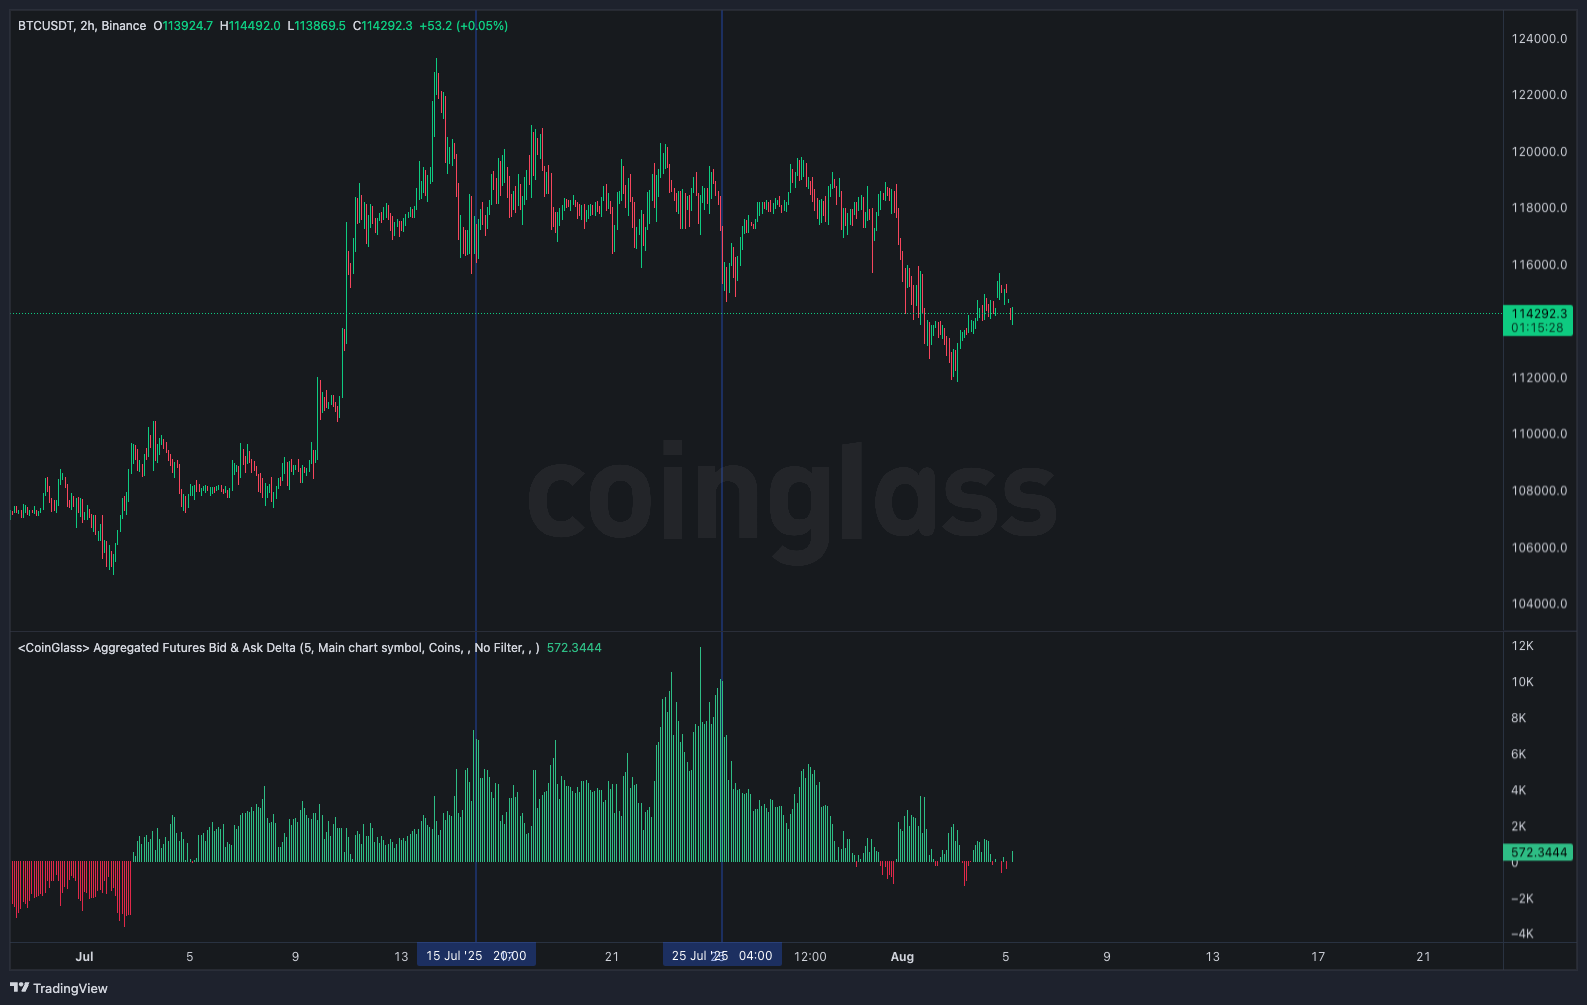
\includegraphics[width=0.95\textwidth]{imgs/showcase_chart.png}
    \caption{Orderbook delta visualization showing price action (top) and corresponding delta values (bottom)}
    \label{fig:orderbook_delta}
\end{figure}

As shown in Figure \ref{fig:orderbook_delta}, the orderbook delta provides valuable insights at extreme values. The chart displays two key components:
\begin{itemize}
    \item The price action (top chart) shows the actual Bitcoin price movements
    \item The orderbook delta (bottom chart) represents the imbalance between buy and sell orders
\end{itemize}

A high orderbook delta value indicates substantial buy orders below the current price. This creates a strong support level, as sellers would need significant pressure to break through these orders. Even if sellers manage to push through, these accumulated buy orders often create buying pressure that can lead to price support or potential rebounds.

This relationship between orderbook delta and price action is particularly useful when:
\begin{itemize}
    \item The delta reaches extreme values, indicating significant order imbalance
    \item There's a clear divergence between price action and orderbook delta
    \item Multiple timeframe analysis shows consistent patterns
\end{itemize}




\newpage
\textbf{Example:}

\begin{verbatim}
    #Example for entry signals in the code
    outlier_mask = (df['trend'] == 'uptrend') & (df['is_outlier'] == 1)
\end{verbatim}

Then I test the strategy on one month of data to evaluate whether it shows any potential. I consider a strategy to have potential if it is around break-even \footnote{Break-even is the point where the total profit equals the total loss. In other words, it's the point where the strategy neither makes nor loses money.} or slightly profitable and achieves a Sharpe ratio between 1 and 2.

\textbf{Results:}

\begin{figure}[H]
    \centering
    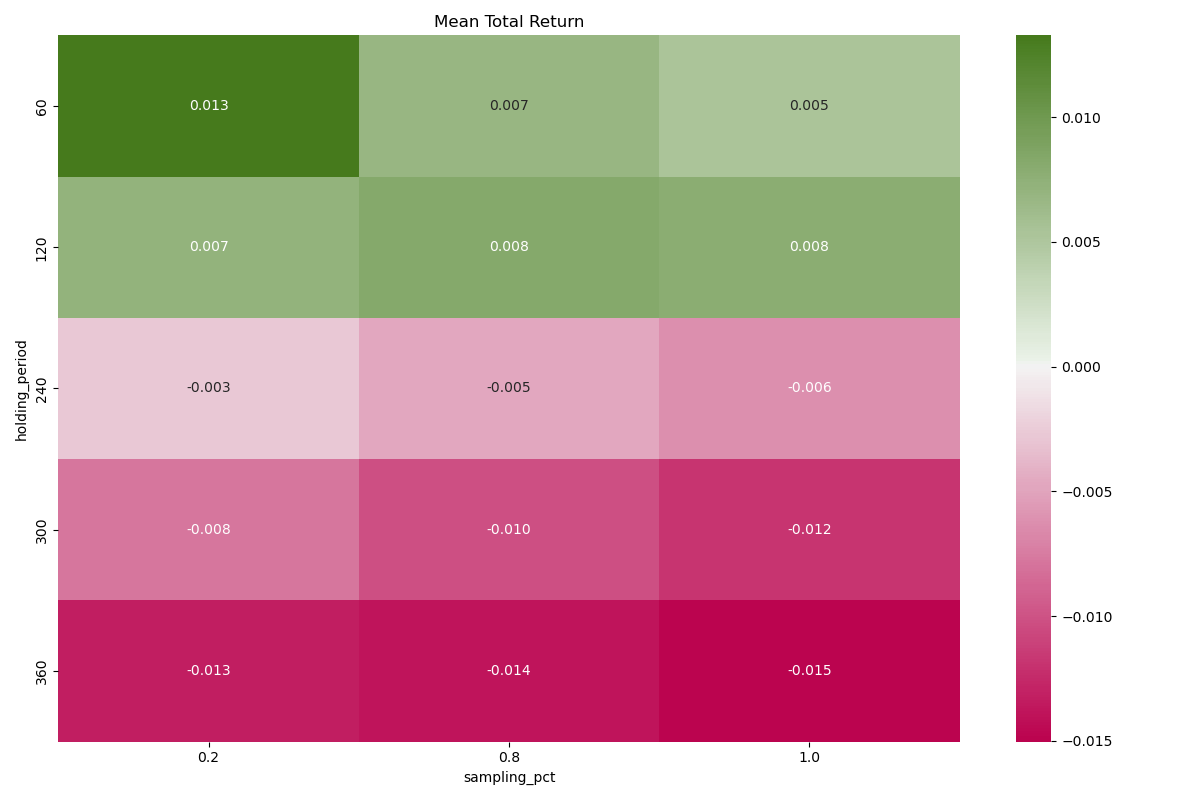
\includegraphics[width=\textwidth,height=0.7\textheight,keepaspectratio]{imgs/showcase_market_simulation.png}
    \label{fig:bullish_outliers_comparison}
\end{figure}

On the $X$ axis you can see the sample size and on the $Y$ axis you can see the average return over he different test runs.



\newpage
\section{Strategy backtest implementation}


\subsection{Sharp ratio}
The sharp ratio will be the main strategy evaluation metric in my backtest
\begin{equation}
    \text{Sharpe ratio} = \frac{\text{Average return $t$}}{\text{Standard deviation $t$} \footnote{$t$ is the time span over which we calculate the average return and the standard deviation} }\cdot \sqrt{98280} \footnote{98280 is used to annualize the Sharpe ratio we do this in order to compare the Sharpe ratio with the Sharpe ratio of other strategies or funds}
\end{equation}


\subsection{Backtesting results}

\begin{itemize}
    \item average sharpe ratio $1.55$ \footnote{The $\overline{SR}$ is the average Sharpe ratio over different walkforward periods}
    \item Over a time period of 137 days a return of $2.7\%$ was achieved
\end{itemize}


\subsection{Backtest parameters}

\begin{itemize}
    \item A stop lost of $2\%$
    \item Exit is 120 minutes after entry or if a regime change occurs
    \item fees of $0.0003\%$ and slippage of $0.0001\%$
    \item accumulate $=$ True \footnote{This allows us to open multiple trades at the same timei}
\end{itemize}


\subsection{Code entry conditions}

\begin{verbatim}
# Entry conditions
entries = (df_temp['outlier_context'] == 'b') & (df_temp['trend'] == 'Uptrend')


# Exit after 120 minutes
time_exit = exitSlots.shift(120).fillna(False)

# Exit on trend change
trendChange = (df_temp['trend'] != df_temp['trend'].shift(1))

#Or statment to exit
exits = trendChange | time_exit
\end{verbatim}




\newpage
\subsection{Entry conditions calculations}
I have to give more context about the entry conditions. $df\_temp$ is just a variable to which I assign a timeseries dataframe \footnote{A dataframe is a two dimensional array with rows and columns} with different kind of metrics inside of it. The entry conditions are defined by two boolean conditions:


\subsubsection{Outlier context}


\begin{verbatim}
    df_temp['outlier_context'] == 'b'
    df_temp['trend'] == 'Uptrend'
\end{verbatim}

As shown in Figure \ref{fig:outlier_context}, the dataframe contains various metrics that we use for our trading decisions:

\begin{figure}[h]
    \centering
    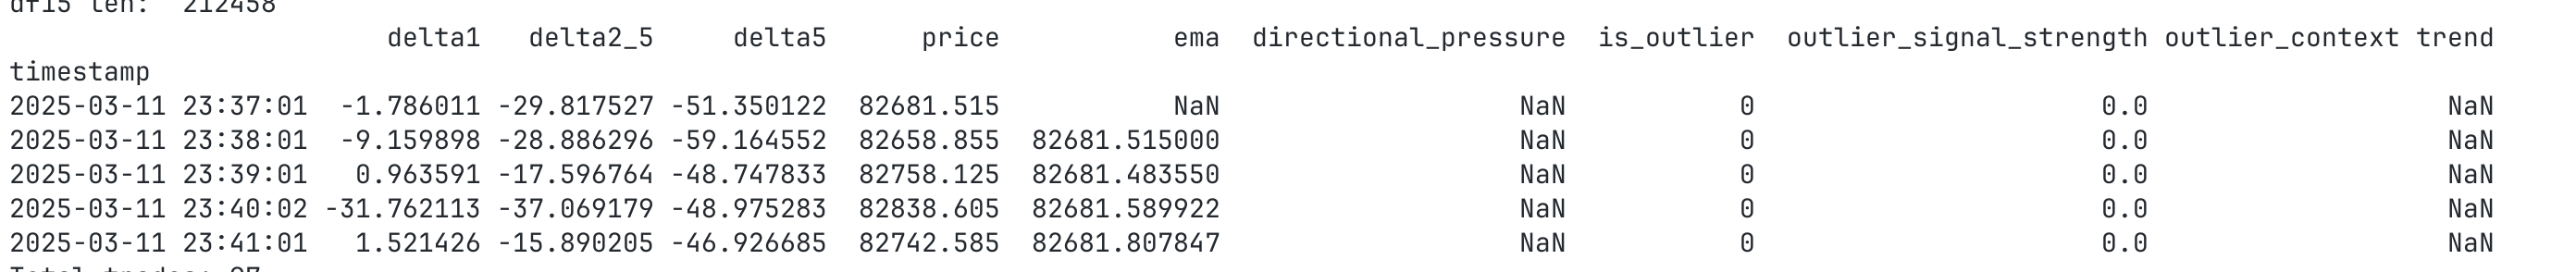
\includegraphics[width=0.95\textwidth]{imgs/dataframeHead.png}
    \caption{}
    \label{fig:outlier_context}
\end{figure}


The column $is\_outlier$ is a binary signal column if the current current orderbook delta value $\Delta_t$ is further than two standard deviations from the mean $\overline{\Delta}_{1440}$ of the orderbook delta.
$outlier\_context$ is a string column that has a value of \textbf{b} if $\Delta_t$ has a postive Z score and \textbf{s} if it has a negative Z score.

\subsection{Market Structure and Trend Identification}

To identify trends in Bitcoin's price, we use a combination of price movement analysis and moving averages. The main challenge is to distinguish between real trends and temporary price movements. We start by converting our 1-minute price data into OHLC \footnote{OHLC stands for Open, High, Low, and Close. It is a type of data that is used to represent the price action of an asset over a period of time and is also known as a candlestick chart.} 240 minute data to better see the overall market direction.

\subsubsection{Price Movement Analysis}
The core of our trend analysis looks at how price moves over time. We use two main indicators:

1. The derivative (rate of change) of a moving average:
\begin{equation*}
    \frac{d}{dt}\text{MA} = \text{Current MA value} - \text{Previous MA value}
\end{equation*}
When this derivative is positive, it indicates an upward trend, and when negative, a downward trend.

2. Price levels comparison:
We compare current prices with previous highs and lows using a window of time ($w$). This helps us confirm if we're really in a trend:
\begin{equation*}
\text{Trend}_t = \begin{cases}
    \text{Uptrend} & \text{if price is making higher highs} \\
    \text{Downtrend} & \text{if price is making lower lows} \\
    \text{Ranging} & \text{otherwise}
\end{cases}
\end{equation*}

\subsubsection{Support and Resistance}
We also look at support and resistance levels to strengthen our trend analysis:

\begin{itemize}
    \item Support: Price levels where buying pressure tends to stop price from falling further
    \item Resistance: Price levels where selling pressure tends to stop price from rising further
\end{itemize}

The slopes of these levels help us determine trend strength. For example, rising support and resistance levels indicate a strong uptrend, while falling levels suggest a downtrend.

\subsubsection{Final Trend Determination}
To make the final decision about the trend, we combine all these factors:
\begin{equation*}
\text{Final Trend} = \begin{cases}
    \text{Uptrend} & \text{if } \frac{d}{dt}\text{MA} > 0 \text{ and making higher highs} \\
    \text{Downtrend} & \text{if } \frac{d}{dt}\text{MA} < 0 \text{ and making lower lows} \\
    \text{Previous Trend} & \text{if moving average confirms} \\
    \text{Ranging} & \text{if no clear direction}
\end{cases}
\end{equation*}

This approach helps us filter out market noise and identify real trading opportunities. We only take trades when all these factors align, which increases our chances of success.





















\newpage
\subsection{Related Work}
Discussion of related work.


\newpage
\section{Methodology}
Your methodology description.



\newpage

\end{document}

